\documentclass[twoside]{article}
\usepackage[all]{xy}
\usepackage{amsmath,amsthm,amssymb,graphicx,tikz,mathrsfs,color,xspace,pdflscape,natbib}
%\usepackage[numbers]{natbib}
\usepackage{fancyhdr}
\usepackage{hyperref}
%%%%%%%%%%%%%%%%%%%% Command for coloring links %%%%%%%%%%%%%%%%%%%%%%%%%%%%%%%
\hypersetup{colorlinks=true,linkcolor=red,citecolor=blue,filecolor=magneta,urlcolor=cyan}
\usepackage{geometry}
\geometry{verbose,a4paper, tmargin=3cm, bmargin=2.5cm, lmargin=3cm, rmargin=3cm, footskip=1.5cm}
\usepackage{times}
\linespread{1.8}
\newtheorem{dfn}{Definition}[section]
\newtheorem{thm}[dfn]{Theorem}
\newtheorem{pro}[dfn]{Proposition}
\newtheorem{rem}[dfn]{Remark}
\newtheorem{lem}[dfn]{Lemma}
\newtheorem{cor}[dfn]{Corollary}
\newtheorem{eg}[dfn]{Example}
\newtheorem{qu}[dfn]{Question}
\newtheorem{con}[dfn]{Construction}
\newtheorem{alg}{Algorithm}
\renewenvironment{proof}{\noindent{\bf Proof. }  \rm } {\hfill{$\Box$}\\}
\renewcommand{\bibname}{References}
\fancyhead[RE]{\thepage}
\fancyhead[LO]{\thepage}
\fancyfoot{\empty} 
\pagestyle{fancy}
\numberwithin{equation}{section}



\newcommand{\U}{\mathcal{U}}
\newcommand{\Sample}{S}
\newcommand{\GFS}{\mathrm{GFS}}
\newcommand{\OGFS}{\mathrm{OGFS}}
\newcommand{\NHT}{\mathrm{NHT}}
\newcommand{\Var}{\operatorname{Var}}
\newcommand{\pr}{\operatorname{Pr}}

\makeatletter
\setlength{\@fptop}{0pt}
\makeatother

\begin{document}
\thispagestyle{empty}

\fancyhead[LE]{Graphical Sampling with MCTS}
\fancyhead[RO]{Panahbehagh and Mohebbi}

\begin{center}
{
\includegraphics [height=25mm, width=\textwidth] {Images/isc18E}} \\
\vspace*{-1.8cm}
\vspace*{4cm}

{\Large \bf Graphical Finite-Population Sampling with Adaptive Monte Carlo Tree Search}\\

{\bf
Bardia Panahbehagh$^1$\footnote[1]{{\bf Corresponding Author:} {\tt bardia.panahbehagh@khu.ac.ir}},
Mehdi Mohebbi$^2$\\
$^1$Faculty of Mathematical Sciences and Computer, Kharazmi University, Tehran, Iran\\
$^2$School of Mathematics, Statistics and Computer Science, University of Tehran, Tehran, Iran}
\end{center}

\noindent\rule{\textwidth}{0.2mm}\par

\noindent{\bf Abstract:}\\
Graphical finite-population sampling represents first-order inclusion probabilities as bars on a unit-height graph. Moving bar segments preserves the prescribed inclusion probabilities, while changing the second-order inclusion probabilities and hence the variance of the Narain--Horvitz--Thompson estimator. This paper presents a short conference version of this framework and studies an adaptive multi-start Monte Carlo tree search for finding lower-variance graphical sampling designs. Numerical results from a tuning experiment show that the method is sensitive to restart and rollout parameters, and that an aggressive restart rule substantially improves the best design found.

\noindent{\bf Keywords:}
Finite-population sampling, graphical sampling, inclusion probabilities, Monte Carlo tree search, Narain--Horvitz--Thompson estimator. \\
\noindent{\bf Mathematics Subject Classification (2010):} $\rm 62D05$, $\rm 62K05$, $\rm 90C59$. \\
\noindent\rule{\textwidth}{0.2mm}\par

\section{Introduction}

Let $\U=\{1,\ldots,N\}$ be a finite population, and let
$\pi_k=\pr(k\in \Sample)$ be prescribed first-order inclusion probabilities
with $0<\pi_k<1$ and $\sum_{k\in\U}\pi_k=E(n_{\Sample})$. For a study
variable $y$, the Narain--Horvitz--Thompson estimator of the population total
$Y=\sum_{k\in\U}y_k$ is
\[
    \widehat Y_{\NHT}=\sum_{k\in \Sample}\frac{y_k}{\pi_k}.
\]
This estimator is unbiased when the first-order inclusion probabilities are
respected. However, its variance depends on the full sampling design through
the second-order inclusion probabilities. Therefore, after fixing the
$\pi_k$'s, an important problem is to construct a feasible design whose
second-order structure gives a small value of $\Var(\widehat Y_{\NHT})$.

Graphical finite-population sampling, introduced by Panahbehagh (2026),
provides a visual and constructive way to address this problem. Each
first-order inclusion probability is represented by a vertical bar of length
$\pi_k$ in the unit interval. A random horizontal line determines the selected
units. Rearranging the bars keeps the first-order probabilities unchanged, but
modifies the joint probabilities. This makes graphical sampling a natural
state space for intelligent search algorithms.

The aim of this paper is to combine graphical sampling with the adaptive
multi-start Monte Carlo tree search (MCTS) implemented in the
{\tt graphical-sampling} package. The algorithm is designed to improve an
initial graphical design according to an exact variance criterion. We summarize
the method and report a compact simulation study based on the tuning results
for the MCTS implementation.

\section{Graphical Finite-Population Sampling}

In graphical finite-population sampling, a design is represented on a
two-dimensional graph. The horizontal axis contains the units
$1,\ldots,N$, and the vertical axis is the interval $[0,1]$. For each unit
$k$, a bar of length $\pi_k$ is placed somewhere in $[0,1]$. A random value
$r\sim U(0,1)$ is drawn, and the sample consists of the units whose bars
intersect the horizontal line at height $r$.

\begin{figure}[ht]
\begin{center}
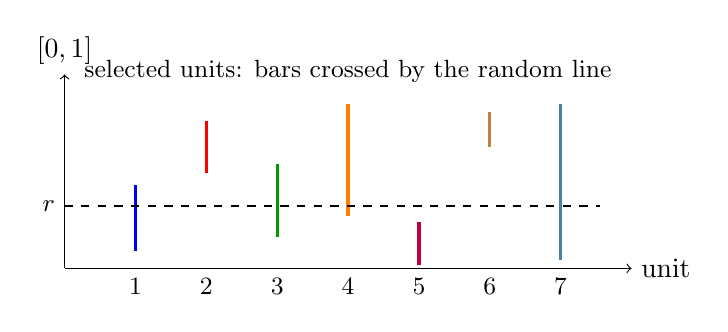
\begin{tikzpicture}[xscale=0.9,yscale=2.2]
  \draw[->] (0,0) -- (8,0) node[right] {unit};
  \draw[->] (0,0) -- (0,1.12) node[above] {$[0,1]$};
  \foreach \x/\a/\b/\c in {1/0.10/0.48/blue,2/0.55/0.85/red,3/0.18/0.60/green!60!black,4/0.30/0.95/orange,5/0.02/0.27/purple,6/0.70/0.90/brown,7/0.05/0.95/cyan!60!black}
    {
      \draw[very thick,\c] (\x,\a) -- (\x,\b);
      \node[below] at (\x,0) {\small \x};
    }
  \draw[dashed,thick] (0,0.36) -- (7.55,0.36);
  \node[left] at (0,0.36) {\small $r$};
  \node[above] at (4.0,1.02) {\small selected units: bars crossed by the random line};
\end{tikzpicture}
\caption{\footnotesize{A graphical sampling design. Each bar has length $\pi_k$.
The random line selects the units whose bars it crosses. Moving bar segments
preserves first-order inclusion probabilities but changes the joint selection
structure.}}\label{fig:gfs}
\end{center}
\end{figure}

The preservation of first-order inclusion probabilities follows immediately:
the probability that the random line crosses the bar of unit $k$ is exactly
the length of the bar, namely $\pi_k$. If the vertical axis is partitioned
into strips with heights $p_1,\ldots,p_T$, each strip corresponds to a sample
$s_t$ and therefore to a sampling design
\[
    p=\{p_t=\pr(\Sample=s_t):t=1,\ldots,T\}.
\]
The second-order inclusion probabilities are then
\[
    \pi_{k\ell}=\sum_{t:k,\ell\in s_t}p_t,\qquad k,\ell\in\U.
\]
For the study variable $y$, the exact design variance can be written as
\begin{equation}\label{eq:nhtvar}
    \Var(\widehat Y_{\NHT})
    =
    \sum_{k\in\U}\sum_{\ell\in\U}
    \frac{y_k y_\ell}{\pi_k\pi_\ell}
    \left(\pi_{k\ell}-\pi_k\pi_\ell\right).
\end{equation}
Thus, within the same vector of inclusion probabilities, different graphical
arrangements can have different precision.

The key operation is to select two strips and move a segment of a bar from
one strip to another vacant position. If the segment length is controlled by
a parameter $\alpha$, this local move keeps the total bar length for every
unit fixed. Consequently, it preserves the first-order inclusion probabilities
while changing the samples and their probabilities. Iterating this operation
produces a large family of feasible designs, including fixed-size designs
when the move is restricted to configurations that preserve sample size.

\section{Adaptive Multi-Start MCTS}

The optimization problem is to find, among feasible graphical designs with
the prescribed $\pi$, a design with small value of the variance criterion
in \eqref{eq:nhtvar}. The implementation studied here uses an adaptive
multi-start MCTS. Each node in the tree stores a graphical design. The reward
of a node is based on the improvement in the best variance value observed
during a rollout.

The tree begins with a virtual root whose children are the initial designs.
At each iteration, the algorithm selects children using the usual upper
confidence principle
\[
    \bar R_j + C\sqrt{\frac{\log N_j}{n_j}},
\]
where $\bar R_j$ is the average reward of child $j$, $n_j$ is its number of
visits, $N_j$ is the number of visits to the parent, and $C$ is the
exploration constant. Expansion creates new children by applying graphical
design mutations. The number of mutations is split between high, middle, and
low magnitudes, with the distribution depending on the previous quality of
the node.

\begin{alg}\label{alg:mcts}
Adaptive multi-start MCTS for graphical sampling designs.
\begin{itemize}
\item Start from one or more valid graphical designs and compute the initial
      variance criterion.
\item Select a tree node by the UCB rule and expand it using high-, mid-, and
      low-magnitude graphical mutations.
\item For each new child, run an adaptive rollout. At every rollout step,
      try an aggressive mutation and, if needed, a conservative mutation;
      retain the better candidate.
\item Stop a rollout early if its current criterion becomes more than
      $15\%$ worse than the initial criterion.
\item Back-propagate the reward
      $100(C_0-C_{\rm best})/C_0$ when an improvement is found, and $0$
      otherwise.
\item If the search stagnates, rebuild the tree from the best design found
      so far.
\end{itemize}
\end{alg}

This structure is useful for graphical sampling because the design space is
large and local moves can easily become trapped. The multi-start root gives
the search several initial directions, rollouts provide short-term local
improvement, and the restart mechanism preserves the best design while
escaping unproductive branches.

\section{Simulation Results}

The simulation report studies the sensitivity of MCTS tuning parameters while
all other settings are fixed. The criterion is the exact NHT variance of the
current graphical sampling design, so smaller values are better. Unless a
parameter is being varied, the baseline settings are 150 iterations, population
size 10, eight children per node, 20 base changes, switch coefficient 1.0,
exploration constant 10, and 18 rollout steps.
The main findings are summarized in Table \ref{tab:tuning}. The values shown
are the best criterion values reported among repeated runs for each tested
setting.

\begin{table}[ht]
\begin{center}
\footnotesize
\caption{Summary of the MCTS tuning experiment. Smaller criterion values are
better.}\label{tab:tuning}
\begin{tabular}{|p{3.2cm}|p{4.7cm}|p{2.0cm}|p{2.4cm}|}
\hline
Parameter & Tested settings & Best setting & Best criterion \\ \hline \hline
Maximum children per node & $5,8,10,15,20$ & $8$ & $163103.34$ \\ \hline
Base changes & $5,10,15,20,25$ & $20$ & $163103.34$ \\ \hline
Switch coefficient & $0.5,0.7,0.9,1.0$ & $1.0$ & $163103.34$ \\ \hline
Exploration constant & $0.5,1.5,5,10,15$ & $10$ & $163103.34$ \\ \hline
Rollout steps & $10,18,30$ & $30$ & $162093.85$ \\ \hline
Population size & $1,10,20,30,40$ & $10$ & $163103.34$ \\ \hline
Early stopping factor & $1.15,1.30,1.50,1.70$ & $1.15$ & $163103.34$ \\ \hline
Restart after no improvement & $3,4,5,8$ & $3$ & $131905.23$ \\ \hline
\end{tabular}
\end{center}
\end{table}

The most important result is the effect of the restart parameter. When the
tree was rebuilt after three non-improving iterations, the best criterion
decreased to $131905.23$, compared with $163103.34$ under the less aggressive
baseline restart. This indicates that stagnation is a major issue in the
graphical-design search space, and that frequent restarts from the best
current design can be more valuable than continuing to expand a stale tree.

The number of children per node also matters. A small value gives too little
breadth, while very large values increase computation without improving the
best criterion. In this experiment, $8$ children per node gave the best
balance. The parameter ${\tt base\_changes}=20$ was also a good setting,
although nearby values produced similar results, suggesting that the adaptive
rollout can compensate for moderate changes in mutation size.

For the switch coefficient, the results favor values near $1.0$; values
$0.5$ and $0.7$ were weaker and often slower. The exploration constant $10$
gave the best reported variance among the tested values, supporting a
relatively exploratory tree policy. Finally, increasing the rollout length
from $18$ to $30$ gave one slightly better criterion value, but at a clear
computational cost. Thus, $18$ rollout steps is a practical compromise, while
$30$ can be used when extra computing time is available.

\section*{Discussion and Conclusion}

Graphical sampling provides a flexible representation of finite-population
sampling designs with fixed first-order inclusion probabilities. The adaptive
multi-start MCTS exploits this representation by searching directly over
feasible graphical designs and using exact NHT variance as the criterion.
The tuning study shows that the method can substantially reduce the criterion,
especially when frequent restarts are used to avoid stagnation. Future work
should compare this MCTS version with A* search, cube sampling, and
determinantal sampling on larger simulated and real populations.

\begin{thebibliography}{99}

\bibitem[Browne et al. (2012)]{Browne2012}
Browne C.B., Powley E., Whitehouse D., Lucas S.M., Cowling P.I., Rohlfshagen P., Tavener S., Perez D., Samothrakis S. and Colton S. (2012), A survey of Monte Carlo tree search methods, {\it IEEE Transactions on Computational Intelligence and AI in Games}, 4(1), 1-43.

\bibitem[Deville and Tille (2004)]{DevilleTille2004}
Deville J.-C. and Tille Y. (2004), Efficient balanced sampling: The cube method, {\it Biometrika}, 91, 893-912.

\bibitem[Horvitz and Thompson (1952)]{HorvitzThompson1952}
Horvitz D.G. and Thompson D.J. (1952), A generalization of sampling without replacement from a finite universe, {\it Journal of the American Statistical Association}, 47, 663-685.

\bibitem[Kocsis and Szepesvari (2006)]{KocsisSzepesvari2006}
Kocsis L. and Szepesvari C. (2006), Bandit based Monte-Carlo planning, {\it Proceedings of the 17th European Conference on Machine Learning}, 282-293.

\bibitem[Loonis and Mary (2019)]{LoonisMary2019}
Loonis V. and Mary X. (2019), Determinantal sampling designs, {\it Journal of Statistical Planning and Inference}, 199, 60-88.

\bibitem[Narain (1951)]{Narain1951}
Narain R.D. (1951), On sampling without replacement with varying probabilities, {\it Journal of the Indian Society of Agricultural Statistics}, 3, 169-174.

\bibitem[Panahbehagh (2026)]{Panahbehagh2026}
Panahbehagh B. (2026), Graphical finite population sampling, {\it Survey Methodology}, 52(1), 129-150.

\bibitem[Panahbehagh et al. (2025)]{GraphicalSampling2025}
Panahbehagh B., Mohebbi M., HosseiniNasab A.M. and Moghadam M.H. (2025), {\it graphical-sampling: A Python package for graphical finite-population sampling}, Python package.

\end{thebibliography}
\end{document}
